% 第 1 章续：块窗口、视图与版图编辑
\section{在块窗口中工作}
\subsection*{Working in the Block Window}

启动 IC Compiler II 并打开 GUI 后，会出现块窗口（block window）。图~\ref{fig:gui-11} 标出块窗口的主要区域。

\begin{figure}[htbp]
\centering
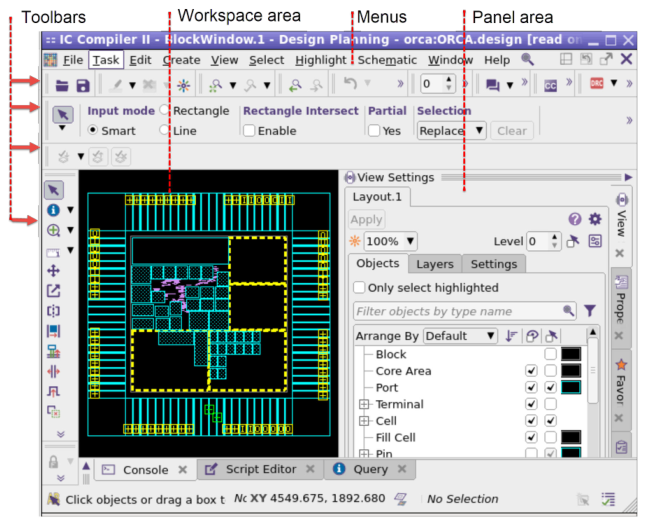
\includegraphics[width=0.92\textwidth]{gui-fig-011.png}
\caption{块窗口的主要功能区}
\label{fig:gui-11}
\end{figure}

打开一个块时，它显示在布局视图（layout view）中，这是该窗口的主块。再打开其他块时，每个块显示在各自的块窗口中。

块窗口是 GUI 的物理设计工作环境。布局视图是查看、分析与编辑块的中心。查看与编辑的细节见后文「更改物理设计的视图」与「编辑物理版图」。

\section{更改物理设计的视图}
\subsection*{Changing the View of the Physical Design}

布局数据往往很密，不同层上的对象互相重叠。可在 View Settings 面板上控制各类对象或各层的可见性（显示或隐藏）与可选性（允许或禁止选择）。也可定制对象或层的属性（颜色、填充图案等），并设置其他布局与对象显示选项。打开多个视图时，可为每个视图设置不同选项。

可用下列方式观察物理版图：
\begin{itemize}
  \item 设置并保存视图属性
  \item 在布局视图中显示网格线
  \item 绘制时序标尺
  \item 绘制物理标尺
  \item 绘制圆形标尺
  \item 用笔势（stroke）激活命令
\end{itemize}

\subsection{设置并保存视图属性}
\subsubsection*{Setting and Saving View Properties}

View Settings 面板用于设置当前活动视图的显示属性，也可把当前设置存入首选项文件，或从该文件加载设置。多个视图可各自使用不同选项。

显示 View Settings 面板：
\begin{itemize}
  \item 选择 \textbf{View > Toolbars > View Settings}；
  \item 或按 F8。
\end{itemize}

若面板被其他面板挡住，在面板区选择 View Settings 选项卡。

该面板可以：
\begin{itemize}
  \item 控制对象或层的可见性与可选性；
  \item 更改颜色、填充图案等样式；
  \item 设置视图或视图中对象的显示选项。
\end{itemize}

图~\ref{fig:gui-12} 是布局视图中对象页的 View Settings 面板。

\begin{figure}[htbp]
\centering
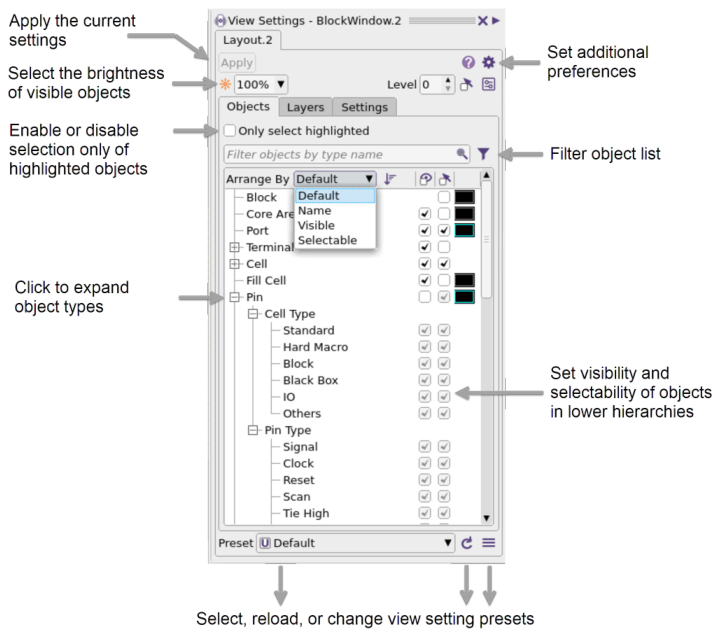
\includegraphics[width=0.85\textwidth]{gui-fig-012.png}
\caption{布局视图中对象的 View Settings 面板}
\label{fig:gui-12}
\end{figure}

设计对象的默认显示特性面向一般观察，对多数块已经合适。若要针对某个块或工作环境定制视图，可按对象类型单独修改。

显示或隐藏特定对象类型或层，可以只看关心的数据。启用或禁止某类对象或某层的选择，可以控制在视图中单击或拖拽时选中哪些对象。

改变样式属性可定制对象外观。可为单个对象类型或层设置颜色、填充图案、轮廓样式、轮廓宽度或夸张（exaggeration）值。

\begin{noteBox}
能改哪些属性，取决于该对象在视图中的图形表示。
\end{noteBox}

可以逐项设置，也可以套用一组预定义视图设置，称为 preset。既可使用工具提供的系统 preset，也可使用自己创建的自定义 preset。详见后文「应用预定义视图设置」。

更改活动布局视图的显示属性：
\begin{enumerate}
  \item 在 View Settings 面板上按需要设置选项。
  \item 单击 Apply。
\end{enumerate}

默认必须单击 Apply 才会生效。也可以让面板在修改后立即自动应用。单击 Options 按钮并选择 Auto apply，即可打开或关闭自动应用。要撤销尚未应用的修改，单击 Options 并选择 Cancel changes。

图~\ref{fig:gui-13} 是单击 Layers 选项卡后、用于设置层选项的面板。

\begin{figure}[htbp]
\centering
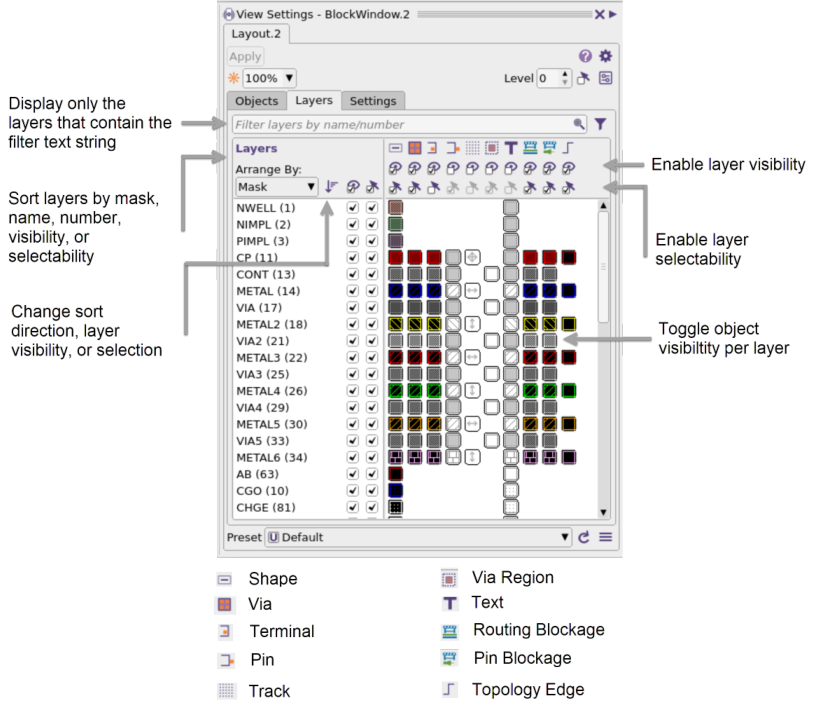
\includegraphics[width=0.85\textwidth]{gui-fig-013.png}
\caption{布局视图中层的 View Settings 面板}
\label{fig:gui-13}
\end{figure}

在层文本过滤框中输入字符串可过滤层列表。键入时，面板只显示名称中包含该文本的层；过滤只影响列表，不改变块窗口中的设计。单击文本框右侧的 (X) 可清除过滤。

单击 Arrange By 并选择排序方式，可按 mask、名称、层名、层号、可见性或可选性重排层列表。默认升序。单击 Arrange By 右侧的箭头可切换排序方向。

图~\ref{fig:gui-14} 是布局视图中 Settings 选项卡。该页有多个子页，用于设置视图、单元、线网、管脚、路径以及掩模颜色的显示选项。

\begin{figure}[htbp]
\centering
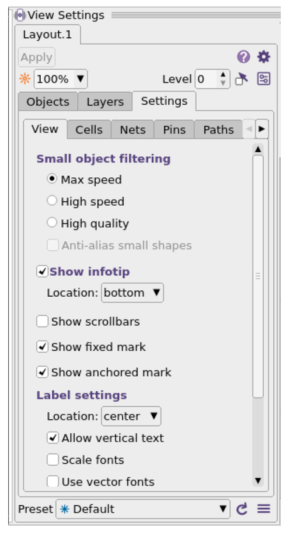
\includegraphics[width=0.55\textwidth]{gui-fig-014.png}
\caption{布局视图 Settings 页的 View Settings 面板}
\label{fig:gui-14}
\end{figure}

\subsubsection{保存与恢复视图设置}
\subsubsection*{Saving and Restoring View Settings}

退出会话时，工具不自动保存视图设置。若希望以后的会话沿用本次修改，可把它们写入首选项文件，之后再从该文件恢复。

保存活动视图的当前设置：在 View Settings 面板单击 Options，选择 \textbf{Preferences > Save To Preferences}。恢复最近一次保存的设置：单击 Options，选择 \textbf{Preferences > Set From Preferences}。

\subsubsection{应用预定义视图设置}
\subsubsection*{Applying Predefined View Settings}

preset 是一组预定义的视图属性。可以使用工具自带的系统 preset，也可以创建并应用自定义 preset。

打开块窗口时，工具默认使用首选项文件中保存的视图设置。要从 preset 应用设置，在 View Settings 面板底部的 Preset 列表中选择该 preset。例如，要套用面向设计规划的系统 preset，选择 floorplan。

在面板上手动改过设置后，Preset 列表中的名称前会出现星号（*）。若要重新套用该 preset 的设置，单击重新加载按钮。要把视图恢复为默认设置，在 Preset 列表中选择 Default。

创建自定义 preset 时要指定名称以及要包含的视图设置。可以新建，也可以重定义已有的自定义 preset，但不能重定义系统 preset。

创建自定义 preset：
\begin{enumerate}
  \item 单击相应按钮并选择 Save preset。出现 Write Layout Setting Preset 对话框。
  \item 选择已有 preset，或在 “Select or type a preset name” 框中输入新名称。
  \item 选择要包含的设置。对布局视图，默认包含 Objects 页的对象类型过滤与对象显示属性、Layers 页的层类型过滤，以及 Settings 页的布局显示设置。还可以选择包含 Layers 页的层显示属性，或 Objects 与 Layers 页的对象样式属性。
  \item 单击 OK。
\end{enumerate}

工具保存该 preset，并把名称加入 View Settings 面板的 Preset 列表。可以把某个 preset 指定为打开新块窗口或新视图时的默认配置。可以删除自定义 preset，不能删除系统 preset。

\subsection{在布局视图中显示网格线}
\subsubsection*{Displaying Grid Lines in a Layout View}

默认不显示网格线。可以显示光刻网格（lithography grid）或用户网格（user grid），以及 FinFET 网格。网格显示后，还可以在默认间距与十倍默认间距之间切换。
\begin{itemize}
  \item 显示或隐藏光刻网格：\textbf{View > Grid > Show Litho Grid}
  \item 显示或隐藏用户网格：\textbf{View > Grid > Show User Grid}
  \item 显示或隐藏 FinFET 网格：\textbf{View > Grid > Show Finfet Grid}
  \item 在默认间距与十倍间距之间切换：\textbf{View > Grid > Cycle grid spacing}
\end{itemize}

\subsection{在布局视图中绘制时序标尺}
\subsubsection*{Drawing Timing Rulers in a Layout View}

时序标尺（timing ruler）用于测量版图中两点之间的时序延时。延时来自 \cmd{read\_parasitic\_tech} 与 \cmd{set\_parasitic\_parameters} 设置的寄生参数，或来自 \cmd{set\_net\_estimation\_rule} 设置的线网估算规则。一条时序标尺可由一段或多段水平或垂直线段组成。默认在每段端点以及段内每第十个刻度处标注从标尺起点起算的延时。

\begin{noteBox}
绘制时序标尺的操作不能用 \textbf{Edit > Undo} 撤销。
\end{noteBox}

绘制步骤：
\begin{enumerate}
  \item 在 Mouse Tools 工具栏单击 Timing Ruler，或选择 \textbf{View > Mouse Tool > Timing Ruler}。启用后，Mouse Tool Options 工具栏出现相应选项，指针形状改变。默认会有十字标尺附着在指针上。
  \item （可选）在 Mouse Tool Options 工具栏设置选项：
  \begin{itemize}
    \item 选择 Attach，把标尺上的点吸附到对象；
    \item 在 Net Estimation Rule 中单击 Use 并选择规则名以计算时序；若不选，则按金属层与缓冲器尺寸计算；
    \item 选择水平层与垂直层；
    \item 更改利用率（utilization）；
    \item 更改缓冲器类型与间距；
    \item 指定非默认布线规则（NDR）；
    \item 更改标尺线段的网格吸附选项。
  \end{itemize}
  \item 在布局视图中单击标尺起点。若已选 Attach，指针经过对象时对象会高亮，标尺吸附到高亮对象。
  \item 单击该段终点。
  \item （可选）重复上述步骤再画一段。
  \item 按 Enter 结束这条标尺。
  \item （可选）重复上述步骤再画另一条标尺。
\end{enumerate}

单击定义标尺之前，可以打开或关闭 Attach，以限制能吸附的对象。可以删除单条标尺或视图中的全部标尺，但不能删除或修改单段线段。删除方法见下一节。

\subsection{在布局视图中绘制物理标尺}
\subsubsection*{Drawing Physical Rulers in a Layout View}

物理标尺用于测量距离，可由一段或多段水平、垂直或对角线段组成。默认在每段端点以及段内每第十个刻度处标注从标尺起点起算的距离。

绘制步骤：
\begin{enumerate}
  \item 在 Mouse Tools 工具栏单击标尺按钮，或选择 \textbf{View > Mouse Tool > Ruler}。启用后出现 Ruler Tool 选项，指针形状改变，默认有十字标尺附着在指针上。
  \item （可选）在 Mouse Tool Options 工具栏设置：
  \begin{itemize}
    \item 标尺模式。默认是两点模式（Two point mode），只画单段；要画多段，选择 Multi point mode；
    \item 方向选项；
    \item 是否显示附着在指针上的十字标尺、从标尺原点到各段端点的距离标签，以及各段中点处的段长标签；
    \item 标签距离的含义：相对设计原点的绝对坐标（Coordinate）、相对标尺原点的距离（Ruler Distance），或相对各段起点的距离（Segment Distance）；
    \item 线段的网格吸附；
    \item 是否把段长或距离记入会话记录（控制台日志）。
  \end{itemize}
  \item （可选）选择 Attach，把起点吸附到对象。
  \item 单击标尺起点。若已选 Attach，指针经过时对象高亮，标尺吸附到高亮对象。
  \item 单击该段终点。
  \item （可选）再画一段。
  \item 按 Enter 结束。
  \item （可选）再画另一条标尺。
\end{enumerate}

这样创建的标尺是持久的：保存设计并重新打开后，自动写入数据库的标尺仍然可用。对持久标尺可以移动、旋转、复制或拉伸。

与 GUI 操作对应的命令如下。

\begin{table}[htbp]
\centering
\caption{标尺相关命令}
\begin{tabularx}{\textwidth}{@{}l l X@{}}
\toprule
操作 & 命令 & 示例 \\
\midrule
新建标尺 & \cmd{create\_ruler} &
\cmd{create\_ruler -name example\_ruler -type ruler -color red -points \{\{123 456\} \{200 200\}\}} \\
查看设计中的标尺 & \cmd{get\_rulers} & \cmd{get\_rulers} \\
删除标尺 & \cmd{remove\_rulers} & \cmd{remove\_rulers} \\
把标注（含标尺）写成 Tcl & \cmd{write\_annotation\_shapes} &
\cmd{write\_annotation\_shapes -file recreate.tcl} \\
\bottomrule
\end{tabularx}
\end{table}

单击定义标尺之前，可以打开或关闭 Attach。可以删除单条或全部标尺，但不能删除或修改单段线段。

删除一条标尺：
\begin{enumerate}
  \item 单击标尺工具，或选择 \textbf{View > Mouse Tool > Ruler}。
  \item 把指针移到要删除的标尺上。
  \item 右键并选择 Remove Nearest Ruler。
\end{enumerate}

删除全部标尺：在 Mouse Tools 工具栏单击相应按钮，或选择 \textbf{View > Mouse Tool > Remove All Rulers}。

\subsection{绘制圆形标尺}
\subsubsection*{Drawing Circular Rulers}

可用 \cmd{gui\_add\_annotation} 创建圆形标尺。详见第~\ref{chap:gui-anno}~章「创建持久标注」。

\subsection{用笔势激活命令}
\subsubsection*{Using Strokes to Activate Commands}

在活动视图中拖动指针画笔势，可以激活预设命令。默认笔势用于：
\begin{itemize}
  \item 放大或缩小块；
  \item 平移块；
  \item 显示整个块。
\end{itemize}

也可以自定义笔势。基本笔势最多 72 种，多段笔势可以更多。

基本笔势是在布局视图中单击中键，或按住中键沿某一方向从一点拖到另一点。配合 Shift、Ctrl 或 Alt（或其组合）时，同一笔势可以激活其他命令。不按修饰键时，典型动作为：单击平移到中心、缩放到全图、矩形放大、矩形缩小等。按住 Ctrl 时，对应动作改为另一组缩放与平移，其中包括缩放到当前选择。

除基本笔势和带修饰键的笔势外，还可以做多段笔势。每一段可以是基本笔势所用的八个方向之一。

把命令绑定到基本或多段笔势，使用 \cmd{set\_gui\_stroke\_binding}。默认 GUI 使用基本笔势而不是多段笔势。用 \cmd{set\_gui\_stroke\_preferences} 可更改该首选项。具体用法见这两个命令的 man 页。

\section{编辑物理版图}
\subsection*{Editing the Physical Layout}

块窗口提供交互工具与命令，用于在库工作区中编辑块的版图。可以：
\begin{itemize}
  \item 移动、改变尺寸、复制和删除对象；
  \item 旋转、翻转对象，并改变单元方向；
  \item 改变对象形状；
  \item 对齐、分布和拉开对象；
  \item 扩展对象；
  \item 创建布线阻挡、线网形状、端口端子、文本对象和通孔。
\end{itemize}

通常先选中要编辑的对象。可以用选择工具交互选择，也可以在 Select By Name 工具栏输入名称。交互编辑工具处于活动状态时也可以选择对象。

选择工具有三种模式：Add、Replace 和 Remove。Add 与 Replace 是默认模式，Remove 是临时模式。按任意加速键可激活某个默认模式。用组合框在 Add 与 Replace 之间切换时，当前模式和默认模式一起改变。用组合框切到 Remove 时，只改变当前模式，默认模式不变，因此随后按键或松开按键会把当前模式恢复为 Add 或 Replace。

编辑工具可通过 Edit 或 Mouse Tools 工具栏上的按钮，或 Edit、Create 菜单打开。图~\ref{fig:gui-15} 给出这些工具栏和 Edit 菜单。相关编辑功能分组放在单击下拉箭头后展开的列表中。

\begin{figure}[htbp]
\centering
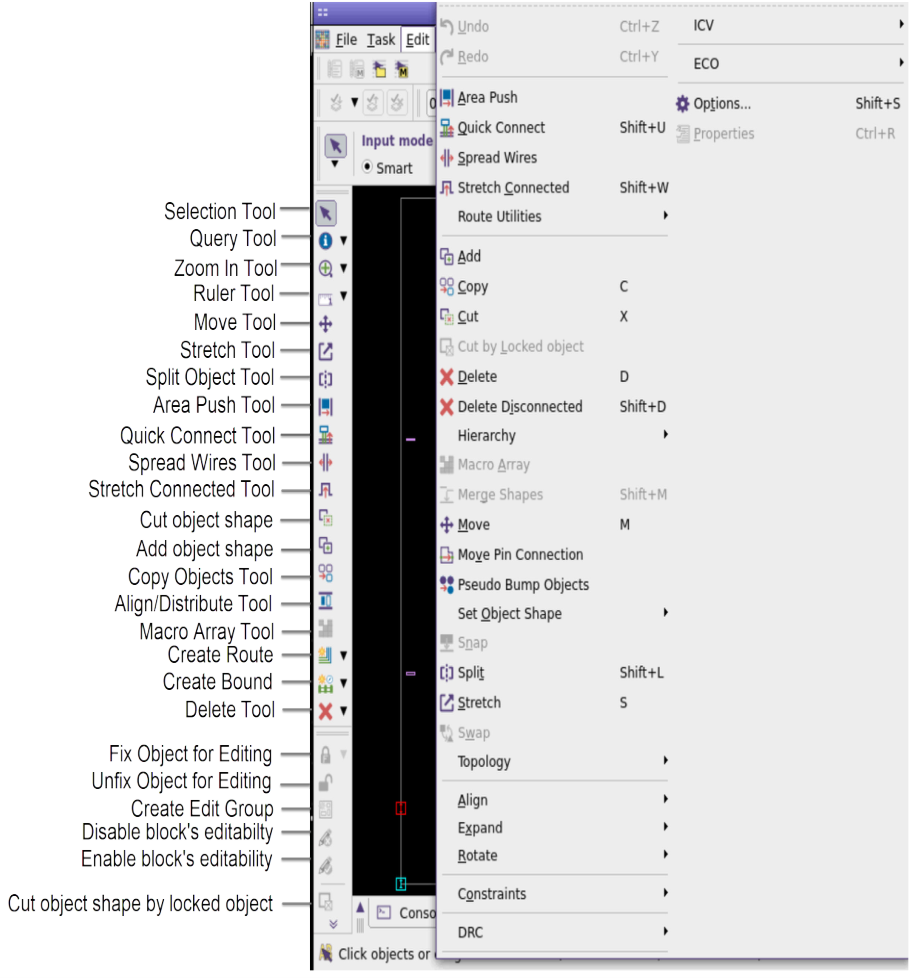
\includegraphics[width=0.92\textwidth]{gui-fig-015.png}
\caption{GUI 编辑命令}
\label{fig:gui-15}
\end{figure}

编辑物理对象与约束的进一步内容：
\begin{itemize}
  \item 交互编辑对象
  \item 在编辑环境中工作
  \item 使用 Editor Toolbox
  \item 使用就地编辑（edit in place）
\end{itemize}

\subsection{交互编辑对象}
\subsubsection*{Editing Objects Interactively}

版图编辑鼠标工具用于在布局视图中交互创建、编辑或删除物理对象。块窗口为所有工具提供一致的编辑环境。可以：
\begin{itemize}
  \item 在 Mouse Tool Options 工具栏设置工具选项；
  \item 用键盘快捷键做频繁或重复的操作；
  \item 预览待选对象，并在重叠对象之间循环。
\end{itemize}

编辑工具处于活动状态时，若要放大、浏览设计或测量距离，可以临时启用 Zoom In、Zoom Out、Pan 或 Ruler，而不必退出编辑工具。

在布局视图中激活某个鼠标工具后，其选项出现在 Mouse Tool Options 工具栏上。

表~\ref{tab:gui-edit-keys} 是交互编辑工具的标准按键。

\begin{table}[htbp]
\centering
\caption{交互编辑工具的按键约定}
\label{tab:gui-edit-keys}
\begin{tabularx}{\textwidth}{@{}X l@{}}
\toprule
动作 & 快捷键 \\
\midrule
单击或拖拽以添加点并执行操作 & Click 或 Drag \\
添加点并应用更改 & Return \\
删除最后一个点 & Backspace \\
取消尚未完成的输入，或退出工具 & Escape \\
在重叠对象中向前循环 & F1 \\
在重叠对象中向后循环 & Shift+F1 \\
撤销最近一次操作 & Ctrl+X \\
重做最近一次已应用的操作 & Ctrl+Y \\
\bottomrule
\end{tabularx}
\end{table}

许多编辑工具作用于已选对象。可以在激活工具之前或之后选择。激活编辑工具时若已有选择，Ctrl+单击把对象加入当前选择，Shift+单击把对象从当前选择中去掉。选中对象以选择色显示，默认是白色。

\begin{noteBox}
若难以选中或预览很小的对象，先放大视图。大设计在低倍率下，有些对象或轮廓小到无法点中。
\end{noteBox}

交互编辑工具能做的操作都会记入日志，并可用 \cmd{gui\_mouse\_tool} 重放。在 Mouse Tool Options 工具栏上设置的选项也会记入日志，并可用 \cmd{gui\_set\_mouse\_tool\_option} 重放。要查看某工具的命令与选项，单击帮助按钮打开该工具的 Help 页。

\subsubsection{移动、修改、创建与删除对象}
\subsubsection*{Moving, Modifying, Creating, and Removing Objects}

可以移动、改变尺寸、复制、拆分、整形、创建和删除对象。表~\ref{tab:gui-edit-tools} 列出常用工具。

\begin{table}[htbp]
\centering
\caption{设计对象的编辑工具}
\label{tab:gui-edit-tools}
\begin{tabularx}{\textwidth}{@{}l X@{}}
\toprule
操作 & 用法 \\
\midrule
移动对象 & \textbf{Edit > Move}，选中对象后单击或拖到新位置 \\
吸附到网格 & \textbf{Edit > Snap} \\
相对锚点对象或位置的边或中心对齐 &
\textbf{Edit > Align > Align/Distribute Tool}，在 Align 页选择对象、指定锚点，再单击对应对齐按钮 \\
相对锚点对象或位置的某一侧分布 &
同一工具的 Distribute 页，指定锚点后单击对应分布按钮 \\
改变尺寸 & \textbf{Edit > Stretch}，拖拽边或角 \\
复制 & \textbf{Edit > Copy}，选中后拖拽 \\
拆分 & \textbf{Edit > Split}，沿拆分位置拖一条线或一个矩形 \\
挖去一块并可选间隙来整形 &
\textbf{Edit > Cut}，可选设置间隙，再在对象上拖出矩形 \\
加上一块并可选间隙来整形 &
\textbf{Edit > Add}，可选设置间隙，再拖出矩形 \\
创建 bound & \textbf{Create > Bound}，拖出矩形 \\
创建布线阻挡 & \textbf{Create > Routing Blockage}，拖出矩形 \\
创建线网形状 & \textbf{Create > Shape}，拖出矩形 \\
创建端子 & \textbf{Create > Terminal}，指定管脚或端口后拖出矩形 \\
创建文本 & \textbf{Create > Text}，指定文字后单击位置 \\
创建通孔或通孔阵列 & \textbf{Create > Via}，单击位置 \\
删除对象 & \textbf{Edit > Delete}，单击或拖出矩形 \\
\bottomrule
\end{tabularx}
\end{table}

上述工具都可在 Mouse Tool Options 工具栏上按需要设置选项。

\subsubsection{扩展与旋转对象}
\subsubsection*{Expanding and Rotating Objects}

\begin{table}[htbp]
\centering
\caption{扩展、旋转与翻转}
\label{tab:gui-edit-xform}
\begin{tabularx}{\textwidth}{@{}l X@{}}
\toprule
操作 & 做法 \\
\midrule
把所选对象向一侧或全部方向扩展 &
单击扩展工具，或选择 \textbf{Edit > Expand > }\textit{direction}；也可使用 \cmd{expand\_objects} \\
将所选对象旋转 90 度或 180 度 &
单击旋转工具，或选择 \textbf{Edit > Rotate}；也可使用 \cmd{rotate\_objects} \\
沿 x 轴或 y 轴翻转 &
单击翻转工具，或选择 \textbf{Edit > Rotate > }\textit{axis}；也可使用 \cmd{flip\_objects} \\
\bottomrule
\end{tabularx}
\end{table}

\subsection{在编辑环境中工作}
\subsubsection*{Working in the Editing Environment}

编辑环境提供增量撤销与重做，可以回退或重新应用最近一次或一系列编辑。编辑时还可以固定（fix）对象、控制网格吸附、设置编辑选项，以及查看和编辑对象属性。表~\ref{tab:gui-edit-global} 是对任何编辑工具都可用的全局操作。

\begin{table}[htbp]
\centering
\caption{全局编辑操作}
\label{tab:gui-edit-global}
\begin{tabularx}{\textwidth}{@{}l X@{}}
\toprule
操作 & 用法 \\
\midrule
撤销上一次编辑 & 单击撤销按钮，或 \textbf{Edit > Undo}，或 \cmd{undo} \\
重做随后的编辑 & 单击重做按钮，或 \textbf{Edit > Redo}，或 \cmd{redo} \\
固定所选对象，避免交互编辑改动它 & \textbf{Edit > Constraints > Fix} \\
取消固定，允许交互编辑改动它 & \textbf{Edit > Constraints > Unfix Edit} \\
启用或关闭网格吸附 &
\textbf{Edit > Options}，在 Snapping 页选中或取消 Snapping enabled \\
查看或编辑所选对象的属性 & \textbf{Edit > Properties} \\
\bottomrule
\end{tabularx}
\end{table}

\subsection{使用 Editor Toolbox}
\subsubsection*{Using the Editor Toolbox}

Editor Toolbox 把移动、旋转、对齐、分布、拉开等常用编辑集中在一处。选择 \textbf{View > Assistants > Editor Toolbox} 打开它，见图~\ref{fig:gui-16}。

\begin{figure}[htbp]
\centering
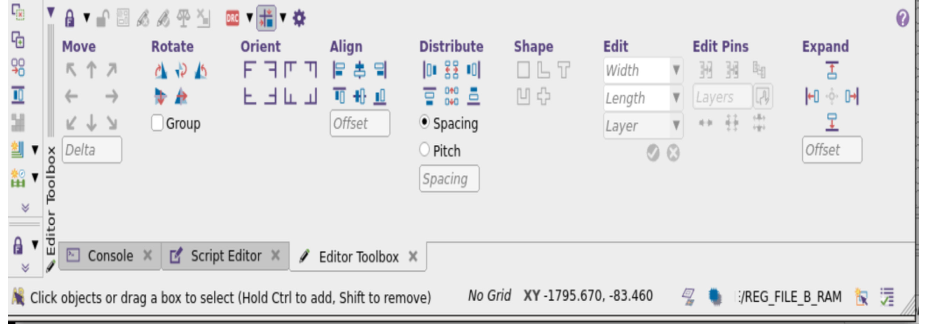
\includegraphics[width=0.92\textwidth]{gui-fig-016.png}
\caption{Editor Toolbox}
\label{fig:gui-16}
\end{figure}

\subsubsection{用 Editor Toolbox 编辑管脚}
\subsubsection*{Editing Pins With the Editor Toolbox}

可用 Editor Toolbox 对块管脚做移动、分布、对齐等操作。

\begin{table}[htbp]
\centering
\caption{管脚编辑操作}
\label{tab:gui-pin-edit}
\begin{tabularx}{\textwidth}{@{}l X@{}}
\toprule
操作 & 用法 \\
\midrule
允许编辑某块上的管脚 &
单击对应按钮，或 \cmd{set\_editability -blocks [get\_selection] -value true} \\
禁止编辑某块上的管脚 &
\cmd{set\_editability -blocks [get\_selection] -value false} \\
合法化所选块管脚，或与所选线网、单元相连的块管脚 &
\cmd{place\_pins -legalize} \\
从当前设计中删除所选端子 & \cmd{remove\_terminals} \\
对齐所选管脚 &
单击对齐按钮。后两个按钮还会分别按层属性改变层宽与层高。对应命令为 \cmd{align\_pins}、\cmd{align\_pins -change\_layer\_width}、\cmd{align\_pins -change\_layer\_height} \\
改变所选管脚宽度 & 在 Edit 区的 Width 框输入新值，单击对勾确认 \\
改变所选管脚长度 & 在 Length 框输入新值后确认 \\
改变所选管脚所在层 & 在 Layer 框选择新层后确认 \\
改变管脚排列 &
选中管脚后单击图标，设为 stacking、interleaving 或 reduce\_crossing。也可在 Design Assistant 的 Pins 页选择管脚，再选 \textbf{Edit > Pin Arrangement} \\
\bottomrule
\end{tabularx}
\end{table}

三种排列方式见图~\ref{fig:gui-17}。

\begin{figure}[htbp]
\centering

\includegraphics[width=0.28\textwidth]{gui-fig-017.png}\hfill
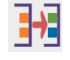
\includegraphics[width=0.28\textwidth]{gui-fig-018.png}\hfill
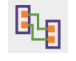
\includegraphics[width=0.28\textwidth]{gui-fig-019.png}
\caption{管脚排列：stacking（左）、interleaving（中）、reduce crossing（右）}
\label{fig:gui-17}
\end{figure}

\subsection{使用就地编辑}
\subsubsection*{Using the Edit in Place Functionality}

就地编辑（edit in place）让你在顶层上下文中编辑子块。它把当前块切换为所选块。可以下推（push）进入所选块，再上弹（pop）回来，也可以设置要查看的层次深度。工具栏见图~\ref{fig:gui-20}。

\begin{figure}[htbp]
\centering
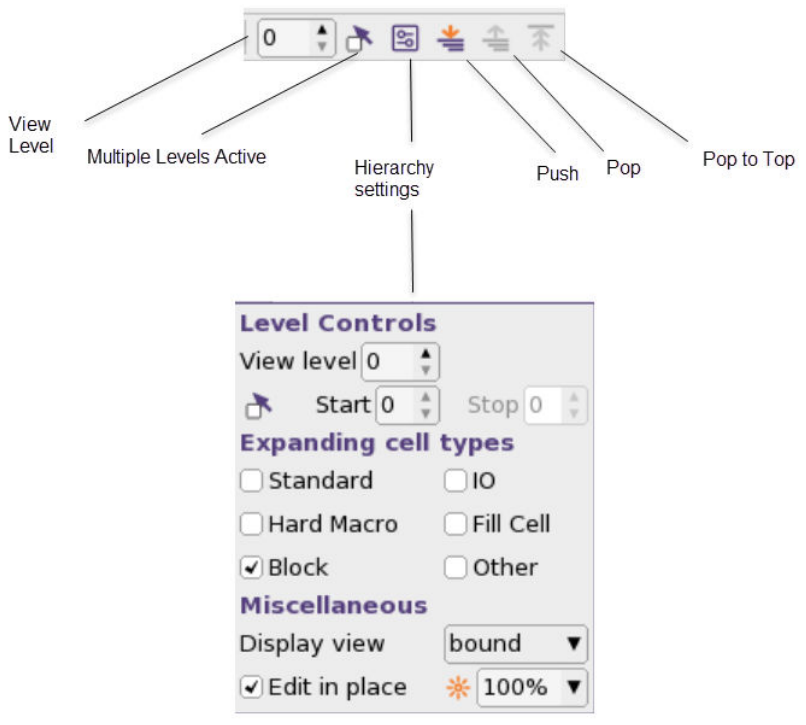
\includegraphics[width=0.92\textwidth]{gui-fig-020.png}
\caption{Edit in Place 工具栏}
\label{fig:gui-20}
\end{figure}

编辑子块：
\begin{enumerate}
  \item 选中要编辑的子块。
  \item 在 Edit in Place 工具栏单击 Push。\\
        下推时工具自动执行 \cmd{set\_working\_design -push}。例如：
\begin{lstlisting}
icc2_shell> set_working_design -push [get_cells \
   I_ORCA_TOP/I_BLENDER_1]
\end{lstlisting}
        可在控制台用 \cmd{current\_block} 核对当前块。
  \item 设计中的其他块会被变暗。用工具中的 dimness 图标调节变暗程度。设为 100\% 则周围块不变暗；设为 Off 则完全隐藏周围块。
  \item 按 F 键全屏缩放到新的当前块。
  \item 在子块上做编辑。
  \item （可选）若设计有多层，可再次 Push，进入更深层的特定对象。
  \item （可选）单击 Pop，向上返回一层。上弹时自动执行 \cmd{set\_working\_design -pop}。
  \item （可选）单击 Pop to Top，回到顶层（level 0）。此时自动执行：
\begin{lstlisting}
icc2_shell> set_working_design -pop -level 0
\end{lstlisting}
  \item （可选）按 Ctrl+F 查看完整设计。
  \item 用 Edit in Place 工具栏改变编辑层次、下推或上弹。
\end{enumerate}

\section{查看金属填充数据}
\subsection*{Viewing Metal Fill Data}

IC Compiler II 支持在同一上下文中编辑设计与金属填充（metal fill）数据。要启用金属填充编辑，打开 View Settings 面板并按图~\ref{fig:gui-21} 修改金属填充设置。金属填充在块内显示为一个或多个填充实例，数据与块一起保存在库中。要编辑这些数据，在 View Settings 面板中启用 All Levels Active。

\begin{figure}[htbp]
\centering
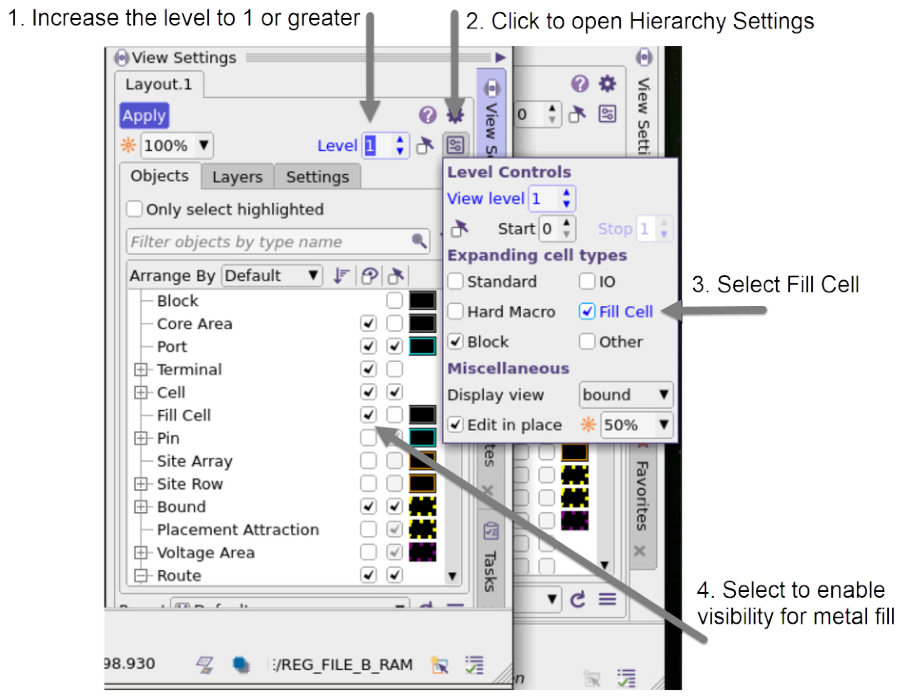
\includegraphics[width=0.85\textwidth]{gui-fig-021.png}
\caption{金属填充显示设置}
\label{fig:gui-21}
\end{figure}
